\documentclass[11pt]{article}
\usepackage[T1]{fontenc}
\usepackage[sc]{mathpazo}
\linespread{1.03}
\usepackage[margin=0.95in]{geometry}
\usepackage{amsmath,amssymb,amsthm,mathtools}
\usepackage{booktabs,tabularx,array}
\usepackage{enumitem}
\usepackage{xcolor}
\usepackage{tikz}
\usetikzlibrary{arrows.meta,positioning,calc}
\usepackage[hidelinks]{hyperref}
\usepackage{microtype}
\usepackage{titlesec}
\usepackage{caption}
\usepackage{needspace}
\captionsetup{font=small,labelfont=bf}

\definecolor{accent}{RGB}{31,94,168}
\definecolor{muted}{RGB}{110,110,110}
\definecolor{boxbg}{RGB}{243,246,250}

% ---------- notation ----------
\newcommand{\R}{\mathbb{R}}
\newcommand{\Pd}{P_\delta}
\newcommand{\Jd}{J_{P_\delta}}
\newcommand{\Uflow}{U_{\mathrm{flow}}}
\newcommand{\Utraj}{U_{\mathrm{traj}}}
\newcommand{\SP}{\mathrm{SP}}
\newcommand{\LB}{\mathrm{LB}}
\newcommand{\ri}{\operatorname{ri}}
\newcommand{\conv}{\operatorname{conv}}
\newcommand{\inshort}[1]{\par\noindent\textcolor{accent}{\textbf{In short.}} #1\par\smallskip}
\newcommand{\std}{\textcolor{muted}{[Standard]}\ }
\newcolumntype{Y}{>{\raggedright\arraybackslash}X}
\setlist{itemsep=1pt,topsep=2pt}
\setlength{\parskip}{4pt}
\setlength{\parindent}{0pt}
\titleformat{\section}{\large\bfseries}{\thesection}{0.6em}{}
\titlespacing*{\section}{0pt}{12pt}{3pt}
\titleformat{\subsection}{\normalsize\bfseries}{\thesubsection}{0.5em}{}
\titlespacing*{\subsection}{0pt}{8pt}{2pt}

\theoremstyle{plain}
\newtheorem{theorem}{Theorem}[section]
\newtheorem{proposition}[theorem]{Proposition}
\newtheorem{lemma}[theorem]{Lemma}
\newtheorem{corollary}[theorem]{Corollary}
\theoremstyle{definition}
\newtheorem{definition}[theorem]{Definition}
\newtheorem{assumption}{Assumption}
\renewcommand{\theassumption}{A\arabic{assumption}}
\theoremstyle{remark}
\newtheorem{remark}[theorem]{Remark}

\begin{document}

{\LARGE\bfseries Certified Trajectory Optimization on Time-Layered Graphs}\\[3pt]
{\large Algorithm proposal, technical version: definitions, theorems and proofs}\\[4pt]
{\color{muted}Zihang Huang \quad·\quad November 3, 2026 \quad·\quad draft}

\vspace{6pt}
\noindent\colorbox{boxbg}{\parbox{\dimexpr\textwidth-2\fboxsep}{
\textbf{The proposal in brief}
\begin{itemize}[leftmargin=1.2em]
  \item \textbf{Goal.} For a contact-rich robot, return a feasible trajectory with cost $U$ and a certified lower bound $L\le J^\star$, with a small gap $U-L$, fast enough to run online.
  \item \textbf{Model.} A time-layered graph (trellis): one layer per time step, one vertex per contact mode. Each edge is one time step in one mode. Its true set is nonconvex. The solver uses a convex outer model of it.
  \item \textbf{Solver.} PDHG on the fractional flow relaxation. Edges update in parallel, prices live on vertices. Most edge solves are skipped exactly. An optional tree pass adds long-range corrections.
  \item \textbf{Lower bound.} From prices alone: a shortest path over per-edge priced minima. It is valid for \emph{any} prices. It is free every round, and tighter when edges are evaluated on their true sets.
  \item \textbf{Upper bound.} Pick mode sequences from the flows and the bound's own paths. Run a local solver along each with the contact schedule fixed.
  \item \textbf{Loop.} Remove edges that provably cannot help, split modes where the gap sits, and repeat until the gap is small.
  \item \textbf{Status.} Every bound is valid by proof. Speed and tightness are empirical.
\end{itemize}}}

\vspace{4pt}
\noindent\fcolorbox{muted}{white}{\parbox{\dimexpr\textwidth-2\fboxsep-2\fboxrule}{\small
\textbf{How to read this version.} The section structure follows the short proposal, with Section~12 on the low-rank segment-tree correction. Each claim is one of three kinds:
\textbf{Theorem / Proposition / Lemma} — proved here (a full proof, or a sketch where marked);
\textbf{\std} — a known result, cited and not reproved;
\textbf{Empirical} — measured, not proved.
Changes from the short draft are listed at the end of the document.}}

%=====================================================================
\section{Problem and setting}
\inshort{Find a good trajectory and prove how good it is.}

\subsection{System}
\begin{itemize}[leftmargin=1.2em]
  \item \textbf{System.} State $x=(q,\dot q)$ of dimension $D$, controls $u$, contact forces $\lambda$, manipulator dynamics $M(q)\ddot q+C(q,\dot q)\dot q+G(q)=Bu+J(q)^\top\lambda$.
  \item \textbf{Contact modes.} $M$ modes (which contacts are active, sticking or sliding). Each mode has its own constraints and dynamics.
  \item \textbf{Horizon.} $N$ time steps of length $\Delta t$, from start $x_0$ to goal set $\mathcal X_g$.
  \item \textbf{One step.} A step in mode $m$ that switches to mode $m'$ is a tuple $w=(x,u,\lambda,x')$ satisfying the discretized dynamics, contact and friction constraints, guards and limits of the pair $(m,m')$.
\end{itemize}

\subsection{The true problem}
\begin{definition}[true problem]\label{def:true}
A \emph{true trajectory} is a mode sequence $m_0,\dots,m_{N-1}$ together with steps $w_k=(x_k,u_k,\lambda_k,x_{k+1})$, $k=0,\dots,N-1$, such that each $w_k$ is a valid step for the pair $(m_k,m_{k+1})$, consecutive steps share their state, $x_0$ is the start and $x_N\in\mathcal X_g$. Its cost is $\sum_k\ell_{(k,m_k,m_{k+1})}(w_k)$. The optimal cost is $J^\star$.
\end{definition}

\subsection{Tolerances and outputs}
\begin{itemize}[leftmargin=1.2em]
  \item \textbf{State tolerance $\delta>0$.} The relaxation lets states disagree at vertices by up to $\delta$ (Section~\ref{sec:form}). True trajectories always agree exactly.
  \item \textbf{Two gaps.} The solver gap $\Uflow-L_\delta\le\eta$ certifies that the relaxation $\Pd$ is solved to accuracy $\eta$. It uses the cost of the current flow (Proposition~\ref{prop:uflow}). The trajectory gap $\Utraj-L_0\le\eta_{\mathrm{traj}}$ certifies a real trajectory. It uses the cost of a local solve (Section~\ref{sec:upper}). The short draft used one symbol for both.
  \item \textbf{Output.} A true trajectory with cost $\Utraj$, and a number $L$ with $L\le J^\star\le\Utraj$.
\end{itemize}

\subsection{Standing assumptions}
\begin{assumption}\label{as:sets}
For every edge $e$: the true set $X_e$ is compact and the true cost $\ell_e$ is lower semicontinuous on it. The outer set $\hat X_e\supseteq X_e$ is nonempty, convex and compact. The outer cost $\hat\ell_e$ is convex and continuous on $\hat X_e$, with $\hat\ell_e\le\ell_e$ on $X_e$.
\end{assumption}
\begin{assumption}\label{as:paths}
After pruning, every edge lies on some path from the start vertex to the goal vertex.
\end{assumption}
\begin{assumption}\label{as:feas}
A true trajectory exists, so $J^\star<\infty$. By Assumption~\ref{as:sets} it is then attained.
\end{assumption}
\begin{assumption}\label{as:delta}
$\delta>0$.
\end{assumption}

%=====================================================================
\section{Formulation: the time-layered trellis}\label{sec:form}
\inshort{A shortest-path problem over modes, with a continuous state carried along each path.}

\subsection{Graph, edges and coupling}
\begin{itemize}[leftmargin=1.2em]
  \item \textbf{Vertices.} $(k,m)$: time step $k\in\{1,\dots,N-1\}$, mode $m$. Plus a start vertex $s$ (layer $0$) and a goal vertex $t$ (layer $N$). $V_k$ is layer $k$.
  \item \textbf{Edges.} $e:(k,m)\to(k+1,m')$ for each allowed transition: about $NM^2$ edges. Write $e^-$ for the tail and $e^+$ for the head. The graph is a DAG whose edges join adjacent layers only.
  \item \textbf{Edge sets.} $X_e\subset\R^{n_e}$ holds the steps $w$ of $e$. Edges out of $s$ fix $x=x_0$; edges into $t$ require $x'\in\mathcal X_g$. Cost $\ell_e$. $X_e$ is \emph{nonconvex} through $M(q)$, $J(q)$, $C$, $G$ and rotations.
  \item \textbf{Coupling maps.} Linear maps $C_e^-,C_e^+:\R^{n_e}\to\R^{d}$ read the coupled coordinates of the pre- and post-state. In the basic formulation $C_e^-w=x$, $C_e^+w=x'$ and $d=D$. A lifted formulation (Section~\ref{sec:optB}) may couple further coordinates, such as second moments of the state. The only requirement is \emph{consistency}: for a true trajectory, $C^+_{e_k}w_k=C^-_{e_{k+1}}w_{k+1}$.
\end{itemize}

\subsection{Perspective sets}
Work with the conic form $Q_e=\{(y,z): y\ge0,\ z\in y\hat X_e\}$. The bound $y_e\le1$ is implied by flow conservation (below), so implementations may add it without changing anything.

\begin{lemma}[perspective]\label{lem:persp}
Under Assumption~\ref{as:sets}, $Q_e$ is a closed convex cone. If $y>0$, then $(y,z)\in Q_e$ if and only if $z/y\in\hat X_e$; if $y=0$, then $z=0$. The perspective cost $\tilde\ell_e(y,z)=y\,\hat\ell_e(z/y)$ for $y>0$, with $\tilde\ell_e(0,0)=0$, is convex, positively homogeneous and continuous on $Q_e$.
\end{lemma}
\begin{proof}
Since $\hat X_e$ is compact, $\{(y,z):y\ge0,z\in y\hat X_e\}$ is closed; the apex case follows from boundedness of $\hat X_e$. Convexity of the perspective of a convex function is standard. Continuity at the apex: $|y\hat\ell_e(z/y)|\le y\max_{\hat X_e}|\hat\ell_e|\to0$.
\end{proof}

Costs can be made linear by the usual epigraph variable, with an upper bound $\max_{\hat X_e}\hat\ell_e$ to keep sets compact. Then $\tilde\ell_e(q_e)=\langle c_e,q_e\rangle$. Sections~\ref{sec:solver} and~\ref{sec:lower} use this form.

\subsection{The relaxation}
For a vertex $v\notin\{s,t\}$, the \emph{state mismatch} is
\[
s_v(q)=\sum_{e:\,e^+=v}C_e^+z_e-\sum_{e:\,e^-=v}C_e^-z_e .
\]
Let $\|\cdot\|$ be a norm on $\R^d$ with dual norm $\|\cdot\|_*$ (the implementation uses $\ell_\infty$, so $\|\cdot\|_*=\ell_1$).

\begin{definition}[relaxation $\Pd$]\label{def:Pd}
\[
\Jd=\min\ \sum_e\tilde\ell_e(y_e,z_e)\quad\text{s.t.}\quad (y_e,z_e)\in Q_e,\quad
\sum_{e^+=v}y_e-\sum_{e^-=v}y_e=\beta_v\ \ \forall v,\quad \|s_v(q)\|\le\delta\ \ \forall v\notin\{s,t\},
\]
with $\beta_s=-1$, $\beta_t=1$ and $\beta_v=0$ otherwise. $P_0$ is the same problem with $\delta=0$.
\end{definition}
On a DAG with unit supply, flow conservation and $y\ge0$ imply $y_e\le1$, and the feasible set is compact.

\begin{theorem}[validity]\label{thm:valid}
Every true trajectory gives a feasible point of $P_0$ (hence of $\Pd$) whose cost is at most the trajectory's cost. Therefore $\Jd\le J_{P_0}\le J^\star$.
\end{theorem}
\begin{proof}
Put $y_e=1$ and $z_e=w_k$ on the trajectory's edges and zero elsewhere. Flow is conserved along the path. Consistency of the coupling maps gives $s_v=0$. Each $w_k\in X_{e_k}\subseteq\hat X_{e_k}$, and $\tilde\ell_{e_k}(1,w_k)=\hat\ell_{e_k}(w_k)\le\ell_{e_k}(w_k)$. Finally $\Jd\le J_{P_0}$ because $\Pd$ has the larger feasible set.
\end{proof}

\textbf{Two sources of gap.} Let $J^{\mathrm{hull}}_{P_\delta}$ denote the relaxation with each $\hat X_e$ replaced by $\conv X_e$ and $\hat\ell_e$ by the convex envelope $\breve\ell_e$ of $\ell_e+\iota_{X_e}$.

\begin{proposition}[gap decomposition]\label{prop:gapdec}
Under Assumption~\ref{as:sets},
\[
J^\star-\Jd=\underbrace{\big(J^\star-J^{\mathrm{hull}}_{P_0}\big)}_{\text{mixing}}+\underbrace{\big(J^{\mathrm{hull}}_{P_0}-J^{\mathrm{hull}}_{P_\delta}\big)}_{\text{tolerance }\delta}+\underbrace{\big(J^{\mathrm{hull}}_{P_\delta}-\Jd\big)}_{\text{convexification}},
\]
and all three terms are nonnegative.
\end{proposition}
\begin{proof}
$\conv X_e\subseteq\hat X_e$, since $\hat X_e$ is convex and contains $X_e$. Also $\hat\ell_e\le\breve\ell_e$ on $\conv X_e$, since $\hat\ell_e$ is convex and lies below $\ell_e$ on $X_e$. So the hull relaxation has a smaller feasible set and a larger objective, which makes the convexification term nonnegative. The tolerance term is nonnegative because enlarging $\delta$ enlarges the feasible set. The mixing term is nonnegative by Theorem~\ref{thm:valid} applied to the hull model.
\end{proof}
Mixing can be positive even when every $X_e$ is convex: flows from different paths average at a vertex, and the averaged state need not be reachable by any single path.

%=====================================================================
\section{Convex outer models for each edge}\label{sec:outer}
\inshort{Exploit the fact that the dynamics are affine in accelerations, torques and forces. Bound the configuration-dependent terms over each mode's region.}

\subsection{Where the nonconvexity is}
Split a step's variables into $\xi=(q,\dot q)$ and $a=(\ddot q,u,\lambda)$. For fixed $\xi$ the dynamics are affine in $a$:
\[
h(\xi,a)=F(\xi)\,a+f(\xi)=0,\qquad F(\xi)a=M(q)\ddot q-Bu-J(q)^\top\lambda,\quad f(\xi)=C(q,\dot q)\dot q+G(q).
\]
All nonconvexity enters through $F$ and $f$. Kinematic and contact constraints have the same structure.

\subsection{Option A: Taylor model with certified band}\label{sec:optA}
Fix a region $\Xi=\{\xi:\|\xi-\bar\xi\|_\infty\le r\}$ and a box $\mathcal A=\{a:\|a-\bar a\|_\infty\le\rho_a\}$, with $\|a\|_\infty\le A$ on $\mathcal A$. For each row $i$, define the constants
\begin{gather*}
c^{f}_{2,i}=\sup_{\xi\in\Xi,\ \|d\|_\infty\le1}\big|D^2f_i(\xi)[d,d]\big|,\qquad
c^{F}_{1,i}=\sup_{\|d\|_\infty\le1,\ \|b\|_\infty\le1}\big|DF_i(\bar\xi)[d]\,b\big|,\\
c^{F}_{2,i}=\sup_{\xi\in\Xi,\ \|d\|_\infty\le1,\ \|b\|_\infty\le1}\big|D^2(F_ib)(\xi)[d,d]\big| .
\end{gather*}
For revolute joints, $F$ and $f$ are trigonometric polynomials in $q$ and polynomial in $\dot q$, so these constants follow from link inertias, joint ranges and velocity limits.

\begin{proposition}[Taylor band]\label{prop:taylor}
Let $h_{\mathrm{lin}}(\xi,a)=F(\bar\xi)a+DF(\bar\xi)[\xi-\bar\xi]\,\bar a+f(\bar\xi)+Df(\bar\xi)[\xi-\bar\xi]$, which is affine in $(\xi,a)$. For all $(\xi,a)\in\Xi\times\mathcal A$ and every row $i$,
\[
\big|h_i(\xi,a)-h_{\mathrm{lin},i}(\xi,a)\big|\ \le\ e_i:=\tfrac12c^f_{2,i}\,r^2+\tfrac12c^F_{2,i}\,A\,r^2+c^F_{1,i}\,r\,\rho_a .
\]
Hence $\hat X^A_e=\{(\xi,a)\in\Xi\times\mathcal A:\ |h_{\mathrm{lin}}(\xi,a)|\le e\}$ (with the edge's other constraints) contains every true step in the region. It is polyhedral if the other constraints are.
\end{proposition}
\begin{proof}
$h-h_{\mathrm{lin}}=\big[F(\xi)-F(\bar\xi)-DF(\bar\xi)[\xi-\bar\xi]\big]a+DF(\bar\xi)[\xi-\bar\xi](a-\bar a)+\big[f(\xi)-f(\bar\xi)-Df(\bar\xi)[\xi-\bar\xi]\big]$. Taylor's theorem with Lagrange remainder bounds the first bracket by $\tfrac12c^F_{2,i}Ar^2$ and the last by $\tfrac12c^f_{2,i}r^2$. The middle term is at most $c^F_{1,i}r\rho_a$.
\end{proof}

\begin{remark}[order of the error]\label{rem:order}
Pure configuration terms ($f$) have error $O(r^2)$. Terms coupling configuration with accelerations, torques or forces ($F(\xi)a$) have an error \emph{first order} in $r$, times the range $\rho_a$ of the affine variables, unless the region also splits $a$. McCormick envelopes of the bilinear terms have the same order (gap $r\rho_a$ for a product over $[\bar\xi_j\pm r]\times[\bar a_l\pm\rho_a]$), but are often tighter. The short draft's ``error scales like (region radius)$^2$'' holds for the first kind only.
\end{remark}

\begin{corollary}[offline sizing]\label{cor:sizing}
A per-edge band $e_i\le\varepsilon$ holds if $r\le\min\{\sqrt{\varepsilon/(c^f_{2,i}+c^F_{2,i}A)},\ \varepsilon/(2c^F_{1,i}\rho_a)\}$ for every $i$. Covering a configuration box of radius $R$ then needs about $(R/r)^{\dim\xi}$ regions. This is exponential in $\dim\xi$, and it is the price of Option A in high dimension.
\end{corollary}

\subsection{Option B: per-edge moment (Shor) relaxation}\label{sec:optB}
Write the edge set as a basic semialgebraic set $X_e=\{w\in\R^n: g_i(w)\ge0,\ h_j(w)=0\}$ with polynomials of degree at most 2. Newton--Euler form makes this possible with a linear number of per-link variables (rotations, twists, wrenches). Add the redundant ball constraint $R^2-\|w\|^2\ge0$, which holds on the compact $X_e$.

\begin{definition}[order-$\kappa$ outer set]\label{def:moment}
Let $m=(m_\alpha)_{|\alpha|\le2\kappa}$ be a moment vector and $L_m$ the Riesz functional. The order-$\kappa$ lifted set $\tilde X_e^{(\kappa)}$ consists of all $m$ with $m_0=1$ and:
\begin{itemize}[leftmargin=1.2em]
  \item the moment matrix $M_\kappa(m)\succeq0$;
  \item localizing matrices $M_{\kappa-\lceil\deg g_i/2\rceil}(g_im)\succeq0$;
  \item $L_m(h_ju)=0$ for every monomial $u$ with $\deg(h_ju)\le2\kappa$;
  \item interval bounds $\underline m_\alpha\le m_\alpha\le\overline m_\alpha$ obtained by interval arithmetic from a box containing $X_e$.
\end{itemize}
Its projection onto first moments is $\hat X_e^{(\kappa)}$. For $\kappa=1$ this is the Shor relaxation: one semidefinite block per edge.
\end{definition}

\begin{proposition}[validity, monotonicity, perspective]\label{prop:moment}
\begin{enumerate}[label=(\roman*),leftmargin=1.6em]
  \item The rank-one moment vector $m(w)=(w^\alpha)_\alpha$ of every $w\in X_e$ lies in $\tilde X_e^{(\kappa)}$. Hence $X_e\subseteq\hat X_e^{(\kappa)}$.
  \item $\hat X_e^{(\kappa+1)}\subseteq\hat X_e^{(\kappa)}$.
  \item Homogenize by replacing $m_0=1$ with $m_0=y\in[0,1]$ and every constant term by $y$. The homogenized set is exactly the closed perspective cone of $\tilde X_e^{(\kappa)}$, and $y=0$ forces $m=0$.
\end{enumerate}
\end{proposition}
\begin{proof}
(i) $M_\kappa(m(w))=vv^\top$ with $v$ the monomial vector; localizing matrices equal $g_i(w)vv^\top\succeq0$; $L_{m(w)}(h_ju)=h_j(w)u(w)=0$; and the interval bounds hold by construction. (ii) The order-$(\kappa+1)$ constraints contain the order-$\kappa$ ones after truncating $m$. (iii) All constraints are linear in $(y,m)$ after homogenization. For $y>0$, dividing by $y$ recovers $\tilde X^{(\kappa)}_e$. For $y=0$ the interval rows give $0\le m_\alpha\le0$.
\end{proof}

\begin{proposition}[convergence to the convex hull]\label{prop:lasserre}
With the ball constraint included, $\hat X_e^{(\kappa)}\to\conv X_e$ in the Hausdorff metric as $\kappa\to\infty$.
\end{proposition}
\begin{proof}
The ball constraint makes the quadratic module Archimedean. Lasserre's theorem \std[Lasserre 2001] then gives, for every $a$, convergence of $\max_{\hat X^{(\kappa)}_e}a^\top w$ down to $\max_{X_e}a^\top w=\sigma_{\conv X_e}(a)$. The support functions are continuous, and they converge monotonically and pointwise on the unit sphere. By Dini's theorem the convergence is uniform. Uniform convergence of support functions is Hausdorff convergence of compact convex sets.
\end{proof}
Finite convergence is not guaranteed in general. No hierarchy over the whole trajectory is needed, because the trellis already separates time steps. Each edge's lift has $\binom{n+2\kappa}{2\kappa}$ moments and a moment matrix of size $\binom{n+\kappa}{\kappa}$, independent of $N$.

\textbf{Lifted coupling.} With Option B the trellis can couple first \emph{and second} moments of the knot state. These coordinates are linear in $m$ and consistent on rank-one points, so Theorem~\ref{thm:valid} applies unchanged.

\subsection{Regions as modes}
A mode can be split into subregions. Each subregion becomes its own mode, with an outer model on the subregion.

\begin{proposition}[refinement is valid and monotone]\label{prop:refine}
Replace a mode by copies on subregions that cover its region. Give each copy's edges outer sets contained in the parent edge's outer set, with costs at least the parent's cost there. Then $\Jd\le\Jd'\le J^\star$, where $\Jd'$ is the refined relaxation.
\end{proposition}
\begin{proof}
\emph{Upper:} every true step lies in some subregion copy, so Theorem~\ref{thm:valid} applies to the refined trellis. \emph{Lower:} map a feasible point of the refined problem to the original by summing, for each original edge, the $(y,z)$ of its copies. The sum lies in the parent's cone $Q_e$, which is a convex cone containing each copy's cone. Flow and state constraints are linear, so they are preserved. The parent's perspective cost is sublinear, being convex and positively homogeneous, so the merged cost is at most the sum of the copies' costs.
\end{proof}

%=====================================================================
\section{Solver core: PDHG on the trellis}\label{sec:solver}
\inshort{Parallel edge steps, price updates on vertices, exact skipping of unnecessary edge solves, and an optional global correction.}

\subsection{Saddle form}
Stack all coupling rows (flow and state) into $Kq-b$. Let $\mathcal D_\delta=\{r:\ r_{\mathrm{flow}}=0,\ \|r_v\|\le\delta\ \forall v\}$ and $g=\iota_{\mathcal D_\delta}$. Then $\Pd$ is $\min_{q\in Q}\langle c,q\rangle+g(Kq-b)$, with Lagrangian
\[
\mathcal L(q,p)=\langle c,q\rangle+\iota_Q(q)+\langle p,Kq-b\rangle-g^*(p),\qquad g^*(p)=\delta\sum_v\|\lambda_v\|_*,
\]
where $p=(p_{\mathrm{flow}},\lambda)$ collects flow prices and state prices.

\begin{lemma}[saddle points exist]\label{lem:saddle}
Under Assumptions~\ref{as:sets}--\ref{as:delta}, $\mathcal L$ has a saddle point. The primal value is $\Jd$, and the dual optimum is attained.
\end{lemma}
\begin{proof}
\emph{Primal:} by Assumption~\ref{as:feas} and Theorem~\ref{thm:valid} the problem is feasible, and the feasible set is compact, so the minimum is attained.

\emph{Constraint qualification:} it suffices to find $q\in\ri Q$ with $Kq-b\in\ri\mathcal D_\delta$ (Fenchel--Rockafellar duality, \std[Rockafellar 1970, Cor.~31.2.1]). Let $\hat q$ be the lift of an optimal true trajectory; its mismatch is zero. For each edge pick $x^\circ_e\in\ri\hat X_e$. By Assumption~\ref{as:paths}, averaging the indicators of finitely many start--goal paths that cover all edges gives a flow $y^u>0$; set $z^u_e=y^u_ex^\circ_e$. For $q_\tau=(1-\tau)\hat q+\tau q^u$ with $\tau\in(0,1]$:
\begin{itemize}[leftmargin=1.2em]
  \item every $y_{\tau,e}>0$;
  \item every $z_{\tau,e}/y_{\tau,e}$ is a convex combination with positive weight on $x^\circ_e$, hence lies in $\ri\hat X_e$ \std[Rockafellar 1970, Thm.~6.1];
  \item flow is conserved exactly;
  \item $\|s_v(q_\tau)\|=\tau\|s_v(q^u)\|<\delta$ for small $\tau$, by Assumption~\ref{as:delta}.
\end{itemize}
So $q_\tau\in\ri Q$ and $Kq_\tau-b\in\ri\mathcal D_\delta$. Duality then gives a zero gap and dual attainment.
\end{proof}

\subsection{One PDHG round}
With positive diagonal step sizes $T$ (primal) and $\Sigma$ (dual):
\begin{align*}
q^{k+1}_e&=\arg\min_{q\in Q_e}\ \langle c_e+K_e^\top p^k,\,q\rangle+\tfrac12\|q-q^k_e\|^2_{T_e^{-1}}\qquad\text{(every edge, in parallel)},\\
p^{k+1}&=\mathrm{prox}_{\Sigma g^*}\big(p^k+\Sigma(K(2q^{k+1}-q^k)-b)\big)\qquad\text{(every vertex, in parallel)}.
\end{align*}
The flow rows are a plain ascent step. The state rows use soft thresholding at $\Sigma\delta$, which is the prox of $\delta\|\cdot\|_1$ (the $\ell_\infty$ case). Pock--Chambolle steps with $\alpha=1$, $T_j=\theta/\sum_i|K_{ij}|$ and $\Sigma_i=1/(\theta\sum_j|K_{ij}|)$, are computed from vertex degrees, so the rule is local. They give $\|\Sigma^{1/2}KT^{1/2}\|\le1$; scaling both by $\rho<1$ makes it strict.

\begin{theorem}[PDHG convergence]\label{thm:pdhg}
\std[Chambolle--Pock 2011; Pock--Chambolle 2011] If a saddle point exists and $\|\Sigma^{1/2}KT^{1/2}\|<1$, the iterates converge to a saddle point. The ergodic averages $\bar z^k$ satisfy a restricted primal--dual gap bound $\mathcal G_B(\bar z^k)\le\big(\|q-q^0\|^2_{T^{-1}}+\|p-p^0\|^2_{\Sigma^{-1}}\big)/(2k)$, uniformly over $(q,p)$ in any bounded set $B$.
\end{theorem}

\begin{lemma}[one round is a proximal-point step]\label{lem:ppa}
\std[He--Yuan 2012] Let $\mathcal A(q,p)=(\partial\iota_Q(q)+c+K^\top p,\ \partial g^*(p)+b-Kq)$, a maximal monotone operator, and
\[
P=\begin{bmatrix}T^{-1}&-K^\top\\-K&\Sigma^{-1}\end{bmatrix}\succ0 .
\]
Then one round is $z^{k+1}=(P+\mathcal A)^{-1}Pz^k$. So the round map $\mathcal T$ is firmly nonexpansive in $\|\cdot\|_P$, and $Pu\in\mathcal A(\mathcal T(w))$ for $u=w-\mathcal T(w)$.
\end{lemma}
\begin{proof}
The primal step's optimality gives $0\in\partial\iota_Q(q^+)+c+K^\top p^+ +T^{-1}(q^+-q)-K^\top(p^+-p)$. The dual step's gives $0\in\partial g^*(p^+)+b-Kq^+ +\Sigma^{-1}(p^+-p)-K(q^+-q)$. Together these read $0\in\mathcal A(z^+)+P(z^+-z)$. A resolvent of a maximal monotone operator in a positive definite metric is firmly nonexpansive in that metric.
\end{proof}

\textbf{Restarts and inexact solves.} Restarts to the average help on sharp problems: for LPs, restarted PDHG converges linearly \std[Applegate et al.\ 2023]. Conic outer models need not be sharp. Edge solves done to a tolerance keep convergence under summability conditions on the errors \std[Rasch--Chambolle 2020].

\subsection{Exact edge skipping}
\textbf{Setting.} The edge step minimizes $\langle g_e,q\rangle+\tfrac12\|q\|^2_{T_e^{-1}}$ over $Q_e$, with \emph{step data} $g_e=c_e+K_e^\top p-T_e^{-1}q_e$. The \emph{pricing value} is $\pi_e(g)=g_y+\min_{x\in\hat X_e}g_x^\top x$: the cost of the cheapest unit-flow transition under data $g$.

\begin{theorem}[zero steps]\label{thm:zero}
The step is $q_e^+=0$ if and only if $\pi_e(g_e)\ge0$.
\end{theorem}
\begin{proof}
Let $\varphi(q)=\langle g_e,q\rangle+\tfrac12\|q\|^2_{T^{-1}}$. For $q=(y,yx)$ with $y>0$, homogeneity gives $\langle g_e,q\rangle=y(g_y+g_x^\top x)\ge y\,\pi_e(g_e)$. If $\pi_e\ge0$, then $\varphi(q)\ge\tfrac12\|q\|^2>0=\varphi(0)$ for every $q\ne0$. If $\pi_e<0$, take a minimizer $x^\star$ and $q_\tau=\tau(1,x^\star)$. Then $\varphi(q_\tau)=\tau\pi_e+O(\tau^2)<0$ for small $\tau>0$.
\end{proof}

\begin{theorem}[dual test]\label{thm:dual}
Let $\hat X_e=\{x:\underline x\le x\le\overline x,\ A_ex-b_e\in\mathcal K_e\}$, with $\mathcal K_e$ a closed convex cone (a product of zero, nonnegative, second-order and PSD cones). For every $\mu\in\mathcal K_e^*$,
\[
\pi_e(g)\ \ge\ \LB_e(g;\mu):=g_y+b_e^\top\mu+\sum_i\min(r_i\underline x_i,\ r_i\overline x_i),\qquad r=g_x-A_e^\top\mu .
\]
Equality holds at an optimal dual of the pricing problem when strong duality holds. For all $g,g'$,
\[
\LB_e(g';\mu)\ge\LB_e(g;\mu)-\|g'-g\|_{B_e},\qquad \|d\|_{B_e}=|d_y|+\textstyle\sum_i|d_i|\max(|\underline x_i|,|\overline x_i|),
\]
and $\pi_e$ is $\|\cdot\|_{B_e}$-Lipschitz.
\end{theorem}
\begin{proof}
For feasible $x$, $\langle\mu,A_ex-b_e\rangle\ge0$, so $g_x^\top x\ge(g_x-A_e^\top\mu)^\top x+b_e^\top\mu$. Minimizing the right side over the box gives the bound. Equality is strong duality. For the perturbation bound, the minimum of $(r+d)^\top x$ over the box is at least the minimum of $r^\top x$ plus the minimum of $d^\top x$. The same argument applied to $\pi_e$ gives the Lipschitz claim.
\end{proof}
\textbf{Use.} Each edge stores one dual vector $\mu_e$. If $\LB_e(g_e;\mu_e)\ge0$, the step is exactly zero and no solver runs. The cost is one pass over the edge's constraint data.

\begin{theorem}[unchanged face]\label{thm:face}
Let $\hat X_e$ be polyhedral, so the step is a strictly convex QP. Fix a set $\mathcal A$ of rows. Solve the KKT equations with the rows in $\mathcal A$ as equalities. If the result satisfies every other row, and its multipliers on the inequality rows of $\mathcal A$ are nonnegative, then it is the step.
\end{theorem}
\begin{proof}
These are the KKT conditions of a convex QP, which are sufficient.
\end{proof}
The KKT matrix depends only on the edge type (mode pair), on $T_e$ and on $\mathcal A$, so one factorization serves every time step with that face and the same steps. For conic edges the analogue is a Newton step on the current face, warm-started from the cached factorization. It is exact only to a tolerance, and convergence then relies on the inexact theory above.

\begin{theorem}[eventually solve-free rounds]\label{thm:solvefree}
Let the iterates converge to $(q^\star,p^\star)$ (Theorem~\ref{thm:pdhg}), with limiting step data $g_e^\star$. Assume:
\begin{enumerate}[label=(\Alph*),leftmargin=1.6em]
  \item every edge with $q^\star_e=0$ has a strict margin $\gamma_e=\pi_e(g^\star_e)>0$;
  \item every polyhedral edge with $q^\star_e\ne0$ has a nondegenerate limiting step: linearly independent active rows and strictly positive multipliers.
\end{enumerate}
Run the rule: zero test; else cached face; else solve. When a zero-centered edge fails its test, refresh $\mu_e$ from the pricing problem. After each step solve, cache the face. Then there is a round $\bar k$ after which no polyhedral edge needs a solve. At every round the iterates equal those of PDHG with exact edge solves.
\end{theorem}
\begin{proof}[Proof sketch]
$g_e^k\to g_e^\star$. \emph{Zero edges:} after a refresh at a round $j$ with $\|g^j_e-g^\star_e\|_{B_e}<\gamma_e/3$, Theorem~\ref{thm:dual} gives $\LB_e(g^k_e;\mu_e)\ge\gamma_e-2\|g^j_e-g^\star_e\|_{B_e}-\|g^k_e-g^\star_e\|_{B_e}>0$ for all later $k$. \emph{Active edges:} under (B), the optimal active set of a parametric QP is locally constant in its data \std[Bemporad et al.\ 2002], so after one solve near the limit the cached face keeps verifying. Iterates are equal because both tests are sound (Theorems~\ref{thm:zero}--\ref{thm:face}).
\end{proof}

\begin{proposition}[when a zero edge costs a solve]\label{prop:whensolve}
An edge with limiting margin $\gamma_e$ whose dual was last refreshed at round $j$ fails its test at round $k$ only if $\gamma_e\le2\|g^j_e-g^\star_e\|_{B_e}+\|g^k_e-g^\star_e\|_{B_e}$.
\end{proposition}
\begin{proof}
At an optimal refresh, $\LB_e(g^j_e;\mu_e)=\pi_e(g^j_e)\ge\gamma_e-\|g^j_e-g^\star_e\|_{B_e}$. Apply the perturbation bound from $g^j_e$ to $g^k_e$, and the triangle inequality.
\end{proof}
\textbf{Accounting identity.} Total solves $=$ step solves (one each time an edge lands on a new face, including switching on or off) $+$ pricing refreshes (one each time a zero-centered edge fails its test). Work is driven by switching events, not by rounds times edges. No bound on the number of switching events before $\bar k$ is claimed.

\subsection{Optional tree pass}\label{sec:tree}
\begin{definition}[frozen-face response]\label{def:Je}
For a polyhedral edge with current active rows $E_e$ and $H_e=T_e^{-1}$, let
\[
J_e=H_e^{-1}-H_e^{-1}E_e^\top(E_eH_e^{-1}E_e^\top)^{+}E_eH_e^{-1}.
\]
\end{definition}

\begin{lemma}[affine response]\label{lem:affine}
$J_e$ is symmetric positive semidefinite. On the critical region where the active set $E_e$ stays optimal, the step is affine in its data: $q^+_e(g)=q^+_e(g_0)-J_e(g-g_0)$. In particular $q^+_e(p)=q^+_e(p_0)-J_eK_e^\top(p-p_0)$ while the face is unchanged.
\end{lemma}
\begin{proof}
$J_e=H^{-1/2}(I-\Pi)H^{-1/2}$, with $\Pi$ the orthogonal projector onto the range of $H^{-1/2}E_e^\top$. With $E_e$ fixed as equalities, the KKT system is linear in $g$ and has a unique primal solution. Eliminating the multipliers gives the stated map \std[Bemporad et al.\ 2002].
\end{proof}

\begin{lemma}[zero-flow edges are invisible]\label{lem:invisible}
If $\pi_e(g_e)>0$, then $q^+_e\equiv0$ on a neighborhood of $g_e$, so the edge contributes nothing to the tree's operator.
\end{lemma}
\begin{proof}
$\pi_e$ is Lipschitz (Theorem~\ref{thm:dual}), so it stays positive nearby, and Theorem~\ref{thm:zero} gives a zero step there.
\end{proof}
This is the precise sense in which the exact tree ``cannot see through edges with zero flow''. It cannot propose activating them.

\begin{proposition}[block tridiagonal by layer]\label{prop:btd}
$S=\sum_eK_eJ_eK_e^\top$ is symmetric positive semidefinite, and $S_{vw}\neq0$ only if $v=w$ or $v,w$ share an edge. Ordering vertex coordinates by layer, $S$ is block tridiagonal. Block $k$ has size $w_k=|V_k|\cdot d'$, with $d'$ the coupled coordinates per vertex ($d'=D+1$ in the basic formulation: one flow and $D$ state coordinates).
\end{proposition}
\begin{proof}
Each term $K_eJ_eK_e^\top$ is PSD and supported on the coordinates of $e^-$ and $e^+$, which lie in adjacent layers.
\end{proof}

\begin{theorem}[cyclic reduction is exact]\label{thm:cr}
Let $S\succ0$ be block tridiagonal with $N$ diagonal blocks of size at most $w$. Odd--even block cyclic reduction computes $S^{-1}r$ exactly, in exact arithmetic, in $2\lceil\log_2N\rceil$ levels. Every pivot block is symmetric positive definite. Work is $O(Nw^3)$; with serial arithmetic inside each merge, depth is $O(w^3\log N)$.
\end{theorem}
\begin{proof}
Given the even layers, the odd layers decouple, because $S$ couples only adjacent layers. Block Gaussian elimination of all odd layers in parallel leaves a block tridiagonal system on the even layers. Its diagonal blocks are Schur complements of an SPD matrix, hence SPD. Recurse ($\lceil\log_2N\rceil$ levels), solve the last block, and back-substitute level by level (the same number of levels). Each level performs $O(\#\text{blocks})$ dense operations of cost $O(w^3)$.
\end{proof}

\begin{proposition}[exact level independence]\label{prop:levels}
Let $S\succ0$ be block tridiagonal by layer. Let $C_l$ be the layers divisible by $2^l$, and call $c$ \emph{new} at level $l$ if $c\in C_l\setminus C_{l+1}$. Let the harmonic shape $\varphi_{l,c}$ be the identity on layer $c$, zero on $C_l\setminus\{c\}$, and of least energy $p^\top Sp$ elsewhere. Collect all shapes of new layers into $\Phi$. Then $\Phi$ is invertible, $\Phi^\top S\Phi$ is block diagonal, and $\Phi(\Phi^\top S\Phi)^{-1}\Phi^\top=S^{-1}$.
\end{proposition}
\begin{proof}
\begin{enumerate}[label=(\roman*),leftmargin=1.6em]
  \item By energy minimization, $S\varphi_{l',c'}$ vanishes outside $C_{l'}$.
  \item A shape $\varphi_{l,c}$ with $c$ new at level $l$ vanishes on $C_{l+1}$.
  \item For $l'>l$: $C_{l'}\subseteq C_{l+1}$, so $\varphi_{l,c}^\top S\varphi_{l',c'}=0$.
  \item At the same level with $c\ne c'$: the supports are separated by a layer of $C_{l+1}$ where both vanish, and $S$ couples only adjacent layers, so the product is again $0$.
  \item Each layer is new at exactly one level, so $\Phi$ is square. Ordered coarse to fine, it is block triangular with identity diagonal blocks, hence invertible.
\end{enumerate}
\end{proof}
This is cyclic reduction written as a basis. A tree node over $[a,b]$ stores the Schur complement of its interior onto layers $a,b$ and the condensed residual.

\begin{proposition}[exact proximal step under frozen faces]\label{prop:newton}
Fix the prox centers $q^k$. Treat as equalities the flow rows and the state coordinates whose $\delta$-bound is active (right-hand side shifted by $\pm\delta$); drop the inactive state coordinates, whose prices are zero. Call the equality rows $(K_E,b_E)$ and let $S_E$ be the corresponding restriction of $S$, assumed positive definite. If every edge's active set is constant on the segment between $p$ and the dual solution $\hat p$ of
\[
\min_{q\in Q}\ \langle c,q\rangle+\tfrac12\|q-q^k\|^2_{T^{-1}}\quad\text{s.t.}\quad K_Eq=b_E,
\]
then $\hat p=p+S_E^{-1}\big(K_Eq^+(p)-b_E\big)$. So one exact tree solve performs one exact primal proximal-point step.
\end{proposition}
\begin{proof}
By Lemma~\ref{lem:affine}, $K_Eq^+(p')-b_E$ is affine in $p'$ on the segment, with slope $-S_E$. The dual optimality condition of the subproblem is $K_Eq^+(\hat p)=b_E$.
\end{proof}
Proximal-point steps converge \std[Rockafellar 1976]. Proposition~\ref{prop:newton} does not bound the number of such steps, nor the number of rounds before the faces settle.

\subsection{Safeguard}\label{sec:safeguard}
A tree direction $d$ is used only behind a test on the round map $\mathcal T$ of Lemma~\ref{lem:ppa}. Write $R(z)=z-\mathcal T(z)$; all norms below are $\|\cdot\|_P$.

\begin{lemma}[a halfspace containing all fixed points]\label{lem:halfspace}
For every $w$ and every fixed point $z^\star$ of $\mathcal T$, $\langle R(w),w-z^\star\rangle_P\ge\|R(w)\|_P^2$.
\end{lemma}
\begin{proof}
$R=I-\mathcal T$ is firmly nonexpansive because $\mathcal T$ is, and $R(z^\star)=0$.
\end{proof}

\needspace{10\baselineskip}
\noindent\fcolorbox{muted}{white}{\parbox{\dimexpr\textwidth-2\fboxsep-2\fboxrule}{\small
\textbf{Algorithm 1 (SuperMann-type safeguard, every step checked).} Input: $z$, $\mathcal T(z)$ (already computed by the ordinary round), a direction $d$ with $\|d\|\le D_{\max}\|R(z)\|$ (rescale otherwise). Parameters $c_1,q\in(0,1)$, $\sigma\in(0,1)$, $\lambda\in(0,2)$, $\beta\in(0,1)$, a trial cap $n_{\max}$, and the state $r_{\mathrm{safe}}$ (initially $\|R(z_0)\|$).
\begin{enumerate}[leftmargin=1.5em,itemsep=0pt]
  \item $\tau\leftarrow1$. Repeat at most $n_{\max}$ times:
  \item \quad $w=z+\tau d$; evaluate $\mathcal T(w)$ (one round of edge work); $R_w=w-\mathcal T(w)$.
  \item \quad \textbf{K1:} if $\|R(z)\|\le r_{\mathrm{safe}}$ and $\|R_w\|\le c_1\|R(z)\|$: accept $z^+=w$, set $r_{\mathrm{safe}}\leftarrow\|R_w\|+q^j$ ($j$ counts K1 steps), stop.
  \item \quad \textbf{K2:} $\rho=\|R_w\|^2-\tau\langle R_w,d\rangle$. If $\rho\ge\sigma\|R_w\|\|R(z)\|$: accept $z^+=z-\lambda(\rho/\|R_w\|^2)R_w$, stop.
  \item \quad $\tau\leftarrow\beta\tau$.
  \item Fallback: $z^+=\mathcal T(z)$, the ordinary step, which is the K2 step with $\tau=0$, $\lambda=1$.
\end{enumerate}
The ``blind'' step of SuperMann (accept $z+d$ without evaluating it) is omitted, so every accepted tree step has been checked against actual edge updates.}}

\begin{theorem}[safeguarded convergence]\label{thm:supermann}
\std[Themelis--Patrinos 2019] With $\mathcal T$ firmly nonexpansive and directions satisfying $\|d_k\|\le D_{\max}\|R(z_k)\|$, the iterates of Algorithm~1 satisfy $R(z_k)\to0$ and converge to a fixed point of $\mathcal T$, i.e.\ a saddle point. If the accepted directions satisfy the Dennis--Moré condition and $R$ is metrically subregular at the limit, the convergence is superlinear.
\end{theorem}
\begin{proof}[Proof sketch]
By Lemma~\ref{lem:halfspace}, a K2 step is a relaxed projection onto a halfspace containing $\mathrm{Fix}\,\mathcal T$, so $\|z^+-z^\star\|^2\le\|z-z^\star\|^2-\lambda(2-\lambda)\rho^2/\|R_w\|^2$. The fallback is a K2 step. K1 steps move at most $D_{\max}\|R(z_k)\|$, and their residuals are summable through the $r_{\mathrm{safe}}$ rule. The sequence is quasi-Fejér, which gives convergence.
\end{proof}

\begin{theorem}[HPE acceptance]\label{thm:hpe}
Let $w=z+\tau d$, $\tilde z=\mathcal T(w)$ and $u=w-\tilde z$, so that $Pu\in\mathcal A(\tilde z)$ by Lemma~\ref{lem:ppa}. If $\|\lambda u+\tilde z-z\|_P\le\sigma\|\tilde z-z\|_P$ with $\sigma\in[0,1)$, then $z^+=z-\lambda u$ satisfies, for every zero $z^\star$ of $\mathcal A$,
\[
\|z^+-z^\star\|_P^2\le\|z-z^\star\|_P^2-(1-\sigma^2)\|\tilde z-z\|_P^2 .
\]
With $d=0$ and $\lambda=1$ the test holds with equality and $z^+=\mathcal T(z)$.
\end{theorem}
\begin{proof}
Monotonicity of $\mathcal A$ gives $\langle u,\tilde z-z^\star\rangle_P\ge0$. Expanding, $\|z^+-z^\star\|^2\le\|z-z^\star\|^2-2\lambda\langle u,z-\tilde z\rangle+\lambda^2\|u\|^2=\|z-z^\star\|^2+\|\lambda u+\tilde z-z\|^2-\|\tilde z-z\|^2$. Then apply the test.
\end{proof}
With $\lambda_k$ bounded below, the $\lambda$-weighted averages of $\tilde z_k$ have restricted gap $O(1/\sum_k\lambda_k)$ \std[Solodov--Svaiter 1999; Monteiro--Svaiter 2010].

\begin{corollary}[the tree pass keeps every guarantee]\label{cor:treesafe}
With either safeguard, PDHG with tree passes converges to a saddle point for any sequence of tree directions (capped as above). The certificate of Section~\ref{sec:lower} is unaffected, because it is valid for any prices.
\end{corollary}

\textbf{Warm starts.} When replanning online, start from the previous cycle's flows, prices, cached faces and stored duals. All results above hold from any starting point; warm starts change only the number of rounds.

%=====================================================================
\section{Lower bound: the certificate}\label{sec:lower}
\inshort{Any prices give a valid bound. It is free to evaluate every round, and evaluating edges on their true sets makes it tighter.}

\subsection{The bound and its validity}
For state prices $\lambda=(\lambda_v)_{v\notin\{s,t\}}$, set $\lambda_s=\lambda_t=0$ and define the edge's priced minimum on a set $Y\in\{\hat X_e,X_e\}$:
\[
\pi_e(\lambda;Y)=\min_{w\in Y}\ \ell(w)+\big\langle C_e^{+\top}\lambda_{e^+}-C_e^{-\top}\lambda_{e^-},\,w\big\rangle,
\]
with $\ell=\hat\ell_e$ on $\hat X_e$ and $\ell=\ell_e$ on $X_e$.

\begin{theorem}[certificate]\label{thm:cert}
For any $\lambda$:
\begin{enumerate}[label=(\roman*),leftmargin=1.6em]
  \item $L_0(\lambda):=\SP[\pi_e(\lambda;\hat X_e)]\ \le\ J_{P_0}\ \le\ J^\star$;
  \item $L_\delta(\lambda):=L_0(\lambda)-\delta\sum_v\|\lambda_v\|_*\ \le\ \Jd$;
  \item $\SP[\pi_e(\lambda;X_e)]\le J^\star$, using the true sets;
  \item each statement remains valid with $\pi_e$ replaced by any lower bound $\underline\pi_e\le\pi_e$.
\end{enumerate}
\end{theorem}
\begin{proof}
\emph{(ii) and (i).} For $q$ feasible for $\Pd$, $\langle\lambda_v,s_v(q)\rangle\ge-\|\lambda_v\|_*\|s_v\|\ge-\delta\|\lambda_v\|_*$. So
$\sum_e\tilde\ell_e(q_e)\ge\sum_e\tilde\ell_e(q_e)+\sum_v\langle\lambda_v,s_v(q)\rangle-\delta\sum_v\|\lambda_v\|_*$.
Regroup the middle sum by edges. Each edge contributes $\phi_e(y_e,z_e)=\tilde\ell_e(y_e,z_e)+\langle C_e^{+\top}\lambda_{e^+}-C_e^{-\top}\lambda_{e^-},z_e\rangle$, which is positively homogeneous, so $\phi_e(y_e,z_e)\ge y_e\,\pi_e(\lambda;\hat X_e)$. The minimum of $\sum_ey_e\pi_e$ over unit start--goal flows on a DAG is attained at a path, because that flow polytope is integral \std[Ahuja--Magnanti--Orlin 1993]. This gives (ii). With $\delta=0$ the $\delta$ term vanishes, which gives $L_0\le J_{P_0}$; then use Theorem~\ref{thm:valid}.

\emph{(iii).} Along a true trajectory, $C^+_{e_k}w_k=C^-_{e_{k+1}}w_{k+1}$ and $\lambda_s=\lambda_t=0$, so the price terms telescope to zero. Hence its cost equals $\sum_k\big[\ell_{e_k}(w_k)+\langle\cdots\rangle\big]\ge\sum_k\pi_{e_k}(\lambda;X_{e_k})\ge\SP[\pi_e(\lambda;X_e)]$.

\emph{(iv).} $\SP$ is monotone in edge costs.
\end{proof}

\begin{remark}[which bound to use]\label{rem:whichL}
$L_\delta$ is the short draft's $L$. It bounds the relaxation $\Pd$ and is the right lower bound for the solver gap. For certifying a trajectory, $L_0\ge L_\delta$ is also valid for $J^\star$ and never smaller. The $\delta$ term is needed only to bound $\Pd$, not $J^\star$.
\end{remark}

\begin{theorem}[no duality gap]\label{thm:nogap}
Under Assumptions~\ref{as:sets}--\ref{as:feas}, $\sup_\lambda L_\delta(\lambda)=\Jd$ for every $\delta\ge0$. Under Assumption~\ref{as:delta} as well, the supremum is attained.
\end{theorem}
\begin{proof}
The partial Lagrangian (state rows dualized, flows kept) is convex--concave and continuous. Its primal domain (perspective cones with conserved unit flow) is compact and convex. Sion's minimax theorem exchanges $\min$ and $\sup$. The inner $\sup_\lambda$ of $\langle\lambda,s\rangle-\delta\|\lambda\|_*$ is the indicator of $\|s\|\le\delta$. The inner $\min$ over flows equals the shortest path, as in the proof of Theorem~\ref{thm:cert}. Attainment for $\delta>0$ follows from Lemma~\ref{lem:saddle}.
\end{proof}

\begin{theorem}[ceiling]\label{thm:ceiling}
For every $\lambda$, $\pi_e(\lambda;X_e)=\min_{w\in\conv X_e}\breve\ell_e(w)+\langle\cdots,w\rangle$. Hence $\SP[\pi_e(\lambda;X_e)]\le J^{\mathrm{hull}}_{P_0}$: no choice of prices, and no evaluation of edges however exact, certifies more than the convex-hull relaxation. Going beyond it requires splitting modes, which changes the graph (Proposition~\ref{prop:refine}).
\end{theorem}
\begin{proof}
Minimizing a lower semicontinuous function plus a linear term over a compact set equals minimizing its closed convex envelope plus the same linear term over the convex hull. Then apply Theorem~\ref{thm:cert}(i) to the hull model.
\end{proof}
Since $\pi_e(\lambda;X_e)\ge\pi_e(\lambda;\hat X_e)$ for every $\lambda$, true-set evaluation never lowers the bound. In particular, at the outer model's optimal prices it gives at least the outer model's value.

\subsection{Every round, no solves}
The certificate uses $g^{\mathrm{cert}}_e(\lambda)=c_e+K_e^\top(0,\lambda)$: no prox center, no flow prices. Flow prices cancel along any start--goal path.

\begin{theorem}[free certificate]\label{thm:free}
For any $\lambda$ and stored $\mu_e\in\mathcal K_e^*$, $\hat L_0(\lambda)=\SP[\LB_e(g^{\mathrm{cert}}_e(\lambda);\mu_e)]\le L_0(\lambda)$, and similarly for $L_\delta$. Equality holds when every $\mu_e$ is optimal at $\lambda$. The cost is one pass over the edges plus one dynamic program, $O(E)$.
\end{theorem}
\begin{proof}
Theorems~\ref{thm:dual} and~\ref{thm:cert}(iv).
\end{proof}
Implementations that split PSD blocks off with edge-local copies and duals $\Lambda_e$ use $\mu_e$'s PSD part $\Gamma_e=\Pi_{\succeq0}(\pm\Lambda_e)$, with the sign set by the splitting convention, so $\mu_e\in\mathcal K_e^*$ holds for any stored values.

\subsection{Lazy exact evaluation}
\begin{theorem}[lazy exact certificate]\label{thm:lazy}
Start from values $v_e=\LB_e\le\pi_e$. Repeat: find a shortest path under $v$; replace $v_e$ by $\pi_e$ on its not-yet-evaluated edges; stop when the path has only evaluated edges. The procedure ends with $\SP[\pi_e]$ exactly. It evaluates only edges whose through-cost under the current values is at most $\SP[\pi_e]$. Stopping early still gives a valid bound.
\end{theorem}
\begin{proof}
Values only increase and stay at most $\pi_e$, so $\SP[v]$ is nondecreasing and at most $\SP[\pi]$. At termination the path $P$ is evaluated, so $\pi(P)=v(P)=\SP[v]\le v(P')\le\pi(P')$ for every path $P'$. Each evaluated edge lay on a path of current value $\SP[v]\le\SP[\pi]$. Termination is finite because each round evaluates at least one new edge.
\end{proof}
In tests this needed about one path's worth of edges.

\subsection{Soundness in floating point}
\begin{proposition}[signed error]\label{prop:signed}
If each computed $\widetilde\LB_e$ satisfies $|\widetilde\LB_e-\LB_e|\le\epsilon_e$, then $\SP[\widetilde\LB_e-\epsilon_e]$ is a valid lower bound. A forward-error bound $\epsilon_e\le\gamma_n\sum|\text{terms}|$ \std[Higham 2002] suffices, computed in the same pass. Bounds from external solvers are used only through their duals in Theorem~\ref{thm:dual}, never through their reported objective values.
\end{proposition}

\subsection{The solver's stopping test on $\Pd$}
\begin{proposition}[flow upper bound]\label{prop:uflow}
If $q$ is feasible for $\Pd$, then $\Uflow(q):=\sum_e\tilde\ell_e(q_e)\ge\Jd\ge L_\delta(\lambda)$ for every $\lambda$. So $\Uflow(q)-L_\delta(\lambda)\le\eta$ certifies that $\Pd$ is solved to accuracy $\eta$.
\end{proposition}
PDHG iterates satisfy flow conservation and conic membership only in the limit. Implementations check them with signed numerical tolerances. The tolerances affect only when the solver stops; $L$ stays rigorous. $\Uflow$ is not a trajectory cost and is never used for the trajectory gap.

%=====================================================================
\section{Upper bound: extracting a trajectory}\label{sec:upper}
\inshort{The relaxation proposes mode sequences and starting points. A local solver makes them exactly feasible.}

\textbf{Candidate mode sequences} (several, solved in parallel):
\begin{itemize}[leftmargin=1.2em]
  \item heaviest paths in the flow's path decomposition;
  \item randomized rounding: sample paths with probability proportional to flow;
  \item the shortest path from the certificate (free each round), and $k$-shortest paths;
  \item greedy: from the start, follow the edge with the most flow.
\end{itemize}

\begin{proposition}[path decomposition]\label{prop:decomp}
\std[Ahuja--Magnanti--Orlin 1993] Every unit start--goal flow on a DAG is a convex combination of at most $|E|$ start--goal paths.
\end{proposition}

\begin{proposition}[rounding has the flow's marginals]\label{prop:round}
Sample a path by starting at $s$ and, at each vertex $v$, taking edge $e$ with probability $y_e/\sum_{e^-=v}y_{e'}$. Then $\Pr[e\in\text{path}]=y_e$ for every edge.
\end{proposition}
\begin{proof}
By induction in topological order, $\Pr[\text{visit }v]$ equals the inflow of $v$, which equals its outflow by conservation. Then $\Pr[e]=\Pr[\text{visit }e^-]\cdot y_e/\mathrm{outflow}(e^-)=y_e$.
\end{proof}
\begin{corollary}\label{cor:roundcost}
With edge states $z_e/y_e$, the expected relaxed cost of a rounded path is $\sum_ey_e\hat\ell_e(z_e/y_e)=\Uflow$. Rounded guesses carry the relaxation's cost on average. What they lack is state agreement at vertices, which the local solver must restore.
\end{corollary}

\textbf{Initialization.} Along the chosen path, use $z_e/y_e$ as the initial guess, or the priced minimizers $\arg\min\pi_e(\lambda)$ when the path came from the certificate.

\textbf{Local solve.} Run a local trajectory optimizer (e.g.\ PHLAME, AGHF, DDP) with the contact schedule fixed. The best feasible result gives $\Utraj$.

\begin{proposition}[when a direct read-off is exact]\label{prop:readoff}
Suppose an optimal solution of $P_0$ has an integral flow (a single path), its edge points lie in the true sets $X_e$, and $\hat\ell_e=\ell_e$ there. Then it is an optimal true trajectory and $J^\star=J_{P_0}$.
\end{proposition}
\begin{proof}
It is a true trajectory, consistent because $s_v=0$, with cost $J_{P_0}\le J^\star$ (Theorem~\ref{thm:valid}).
\end{proof}
This is rare when flows mix, which is why the local solve is part of the method.

%=====================================================================
\section{Screening and refinement}\label{sec:screen}
\inshort{Remove what provably cannot help. Refine where the gap actually is.}

\begin{theorem}[safe screening]\label{thm:screen}
Fix $\lambda$ and edge values $v_e\le\pi_e(\lambda;X_e)$, for instance $v_e=\LB_e$. Let $d_s(\cdot)$ and $d_t(\cdot)$ be the shortest-path distances from the start and to the goal under $v$, and $\tau_e=d_s(e^-)+v_e+d_t(e^+)$. Every true trajectory using $e$ costs at least $\tau_e$. So if $\tau_e>\Utraj$ for some true trajectory's cost $\Utraj$, no optimal trajectory uses $e$, and removing it is safe. The removal is permanent: it stays valid as $\Utraj$ decreases. The relaxation of the reduced graph has value in $[\Jd,J^\star]$.
\end{theorem}
\begin{proof}
For a true trajectory through $e$, the price terms telescope, as in Theorem~\ref{thm:cert}(iii). Its cost is therefore at least the $v$-length of its path, which is at least $\tau_e$. Removing edges shrinks the feasible set, so the value cannot decrease. The optimal trajectory (attained by Assumption~\ref{as:feas}) survives, so the value is at most $J^\star$.
\end{proof}
No $\delta$ term is needed in $\tau_e$, because true trajectories agree exactly at vertices.

\textbf{Mode refinement.} Split a mode's region where the outer model is loose: where an edge's true priced minimum differs most from its outer-model value, or where flows mix. Proposition~\ref{prop:refine} guarantees the bound cannot get worse. By Proposition~\ref{prop:taylor}, halving $r$ quarters the configuration part of the Option A band and halves the bilinear part. The effect on mixing is empirical.

\begin{theorem}[when factoring is exact]\label{thm:factor}
Factoring splits each layer into $M$ dynamics edges into new vertices $(k+\tfrac12,m)$ followed by $M^2$ switch edges that copy the state, apply the target mode's constraints and pay the switching cost. Suppose that for each source mode $m$:
\begin{itemize}[leftmargin=1.2em]
  \item the dynamics are $x'=A_mx+B_mu+c_m$ with $A_m$ invertible;
  \item the control set and a convex control cost depend only on $m$;
  \item pair-specific constraints act only on $x'$.
\end{itemize}
Keep the first layer unfactored. Then the factored relaxation has the same value as the original relaxation \emph{without} per-copy pre-state constraints.
\end{theorem}
\begin{proof}[Proof sketch]
Pooling the copies of the original gives a factored point, by convexity. Conversely, give every copy the pooled control. Invertibility of $A_m$ lets each copy's pre-state be solved for, and these average to the pooled pre-state. That requires free pre-state copies, which is why the pinned first layer stays unfactored.
\end{proof}
\textbf{Empirical:} factoring cut heavy solves by $M\times$ and gave a $0.5$--$30\%$ looser bound than the standard relaxation in tests. Use it only if the solve count dominates.

%=====================================================================
\section{The full loop}
\begin{center}
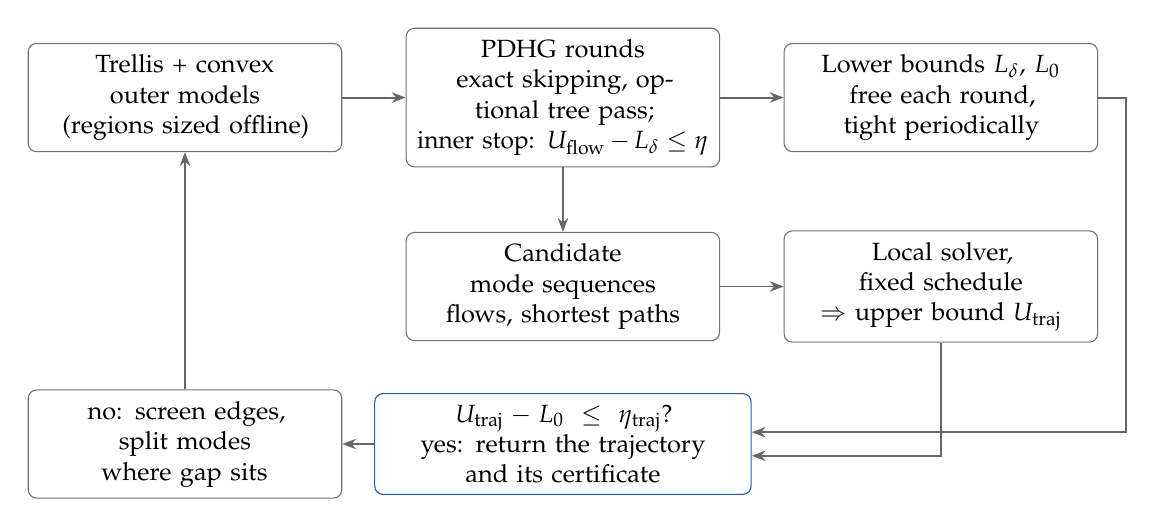
\begin{tikzpicture}[
  b/.style={draw=black!55,rounded corners=3pt,align=center,font=\small,inner sep=4pt,fill=white,text width=3.7cm},
  a/.style={-{Stealth[length=5pt]},black!60,line width=0.7pt}]
  \node[b] (m) at (0,0) {Trellis + convex outer models\\(regions sized offline)};
  \node[b] (p) at (4.8,0) {PDHG rounds\\exact skipping, optional tree pass;\\inner stop: $\Uflow-L_\delta\le\eta$};
  \node[b] (l) at (9.6,0) {Lower bounds $L_\delta$, $L_0$\\free each round, tight periodically};
  \node[b] (c) at (4.8,-2.4) {Candidate mode sequences\\flows, shortest paths};
  \node[b] (u) at (9.6,-2.4) {Local solver, fixed schedule\\$\Rightarrow$ upper bound $\Utraj$};
  \node[b,draw=accent,text width=4.5cm] (g) at (4.8,-4.4) {$\Utraj-L_0\le\eta_{\mathrm{traj}}$?\\yes: return the trajectory\\and its certificate};
  \node[b] (r) at (0,-4.4) {no: screen edges,\\split modes where gap sits};
  \draw[a] (m) -- (p); \draw[a] (p) -- (l); \draw[a] (p) -- (c); \draw[a] (c) -- (u);
  \draw[a] (u.south) |- ($(g.east)+(0,-0.15)$);
  \draw[a] (l.east) -- ++(0.35,0) |- ($(g.east)+(0,0.15)$);
  \draw[a] (g) -- (r);
  \draw[a] (r) -- (m);
\end{tikzpicture}
\end{center}

\needspace{14\baselineskip}
\noindent\fcolorbox{muted}{white}{\parbox{\dimexpr\textwidth-2\fboxsep-2\fboxrule}{\small
\textbf{Algorithm 2.}
\begin{enumerate}[leftmargin=1.5em,itemsep=0pt]
  \item \textbf{Offline:} build the trellis; size mode regions for the target per-edge error (Corollary~\ref{cor:sizing}); precompute outer models and shared factorizations.
  \item \textbf{Initialize:} flows, prices, caches and duals from the previous cycle, or zero on a cold start.
  \item \textbf{Repeat} PDHG rounds. In each round: (a) zero test, else cached face, else solve, for every edge in parallel; (b) price update; (c) optionally, a tree pass behind the safeguard (Algorithm~1); (d) free lower bounds (Theorem~\ref{thm:free}). The inner loop has done its job when $\Uflow-L_\delta\le\eta$ (Proposition~\ref{prop:uflow}).
  \item \textbf{Every few rounds:} tighten the bounds with true-set edge evaluations, lazily along shortest paths (Theorem~\ref{thm:lazy}); extract candidate mode sequences; run local solves in parallel; update $\Utraj$.
  \item \textbf{Stop} when $\Utraj-L_0\le\eta_{\mathrm{traj}}$, or when the time budget ends; return the best trajectory and the current certificate.
  \item \textbf{Otherwise,} when progress stalls: screen edges against $\Utraj$ (Theorem~\ref{thm:screen}); split modes where the gap concentrates; continue from the current state.
\end{enumerate}}}

%=====================================================================
\section{What is guaranteed, and what is not}
\begin{center}
\small
\begin{tabularx}{\textwidth}{@{}>{\raggedright\arraybackslash}p{5.0cm}>{\raggedright\arraybackslash}p{2.6cm}Y@{}}
\toprule
Claim & Status & Note \\
\midrule
$L_0\le J^\star$ and $L_\delta\le\Jd$ at every round & Thm~\ref{thm:cert}, \ref{thm:free} & Any prices; any valid per-edge bounds; signed numerical error (Prop.~\ref{prop:signed}) \\
Bounds can reach $\Jd$ & Thm~\ref{thm:nogap} & At optimal prices; ceiling $J^{\mathrm{hull}}_{P_0}$ (Thm~\ref{thm:ceiling}) \\
$\Utraj$ is a real trajectory's cost & By construction & Checked by the local solver's feasibility \\
PDHG converges on outer models & Thm~\ref{thm:pdhg} (Std.) & $O(1/k)$ ergodic restricted gap; saddle point exists (Lemma~\ref{lem:saddle}) \\
Rounds: $N\lesssim R$; dual size $\le(U-L')/\delta$ & Prop.~\ref{prop:local}, \ref{prop:dualsize} & Upper end via the ergodic rate; pessimistic \\
Edge skipping changes nothing & Thm~\ref{thm:zero}--\ref{thm:face} & Polyhedral edges exactly; conic edges to tolerance \\
Eventually no edge solves & Thm~\ref{thm:solvefree} & Needs strict complementarity and nondegeneracy \\
Tree pass: exact linear solve, safeguarded & Thm~\ref{thm:cr}, Cor.~\ref{cor:treesafe} & Speed-up only once active sets settle (Prop.~\ref{prop:newton}) \\
Low-rank tree: consistent, safeguarded & Thm~\ref{thm:consistent}, Cor.~\ref{cor:lowrank} & Usefulness of the correction is empirical \\
Screening is safe & Thm~\ref{thm:screen} & Removal is permanent and only tightens \\
Gap size $U-L$ & Empirical & Ceiling: per-edge convex hulls plus mixing (Prop.~\ref{prop:gapdec}) \\
Rounds to reach $\eta$ & Empirical & No general bound beyond the bracket below \\
Solve savings at real scale & Empirical & Edge size changes how often faces switch \\
\bottomrule
\end{tabularx}
\end{center}

\begin{proposition}[locality floor]\label{prop:local}
In PDHG without tree passes and without global restart decisions, started from zero, the prices after $k$ rounds at layers $\le j$ depend only on the problem data at layers $\le j+k+1$. Hence, for any family of instances that differ only near the goal but whose $\Pd$ solutions differ near the start by more than a tolerance $\varepsilon$, at least about $N$ rounds are needed to reach accuracy $\varepsilon$ on all of them.
\end{proposition}
\begin{proof}
An edge step uses prices at its two endpoint layers. A price update uses edges incident to its vertex. So the dependence radius grows by one layer per round, by induction.
\end{proof}
The tree pass reaches the whole horizon in $2\lceil\log_2N\rceil$ levels, so the floor does not apply to PDHG with tree passes.

\begin{proposition}[size of optimal prices]\label{prop:dualsize}
Let $U$ be the cost of any true trajectory and $L'$ any lower bound on $\Jd$. Every optimal state price $\lambda^\star$ of $\Pd$ satisfies $\delta\sum_v\|\lambda^\star_v\|_*\le U-L'$.
\end{proposition}
\begin{proof}
Let $\hat q$ be the trajectory's lift, which has $s_v(\hat q)=0$. By Theorem~\ref{thm:nogap}, $\Jd=L_\delta(\lambda^\star)\le\sum_e\tilde\ell_e(\hat q_e)+\langle\lambda^\star,s(\hat q)\rangle-\delta\sum_v\|\lambda^\star_v\|_*\le U-\delta\sum_v\|\lambda^\star_v\|_*$.
\end{proof}
Combined with Theorem~\ref{thm:pdhg}, with step sizes balanced as $\tau\propto R_x/(R_p\|K\|)$ and $\sigma\propto R_p/(R_x\|K\|)$, the ergodic restricted gap falls below $\eta$ after about $\|K\|R_xR_p/\eta$ rounds. Here $R_x$ is the primal diameter, and $R_p$ bounds the optimal prices: the state part by Proposition~\ref{prop:dualsize}, and the flow part by shortest-path potentials. This is a bound on the restricted gap, not on the certificate gap. It depends on $1/\delta$ and is pessimistic. The time before active sets settle is not bounded.

%=====================================================================
\section{Cost model}
\begin{itemize}[leftmargin=1.2em]
  \item \textbf{Per round:} one cheap pass over all $E\approx NM^2$ edges (a dot product or a small matrix--vector product each); genuine solves only at switching events; one price update; one $O(E)$ shortest path.
  \item \textbf{Periodic:} true-set edge bounds along shortest paths; local solves for a few candidates, in parallel.
  \item \textbf{Exact tree pass:} $O(Nw^3)$ work in $2\lceil\log_2N\rceil$ levels, with $w=M(D+1)$ in the basic formulation; at most about one round of edge solves at full width.
  \item \textbf{Low-rank tree pass:} $O(N[wr^2+r^3])$ internal work, plus reference setup and application costs (Section~\ref{sec:lowrank}).
  \item \textbf{Wall-clock:} $T\approx\sum_{\text{rounds}}\big(\text{cheap pass}+\lceil\text{solves}/P\rceil\,C\big)+T_{\text{bounds}}+T_{\text{local}}$, with $P$ the parallel capacity and $C$ one edge solve.
  \item \textbf{Empirical,} small polyhedral test ($D=2$, $M=4$--$8$, $N=20$):
  \begin{itemize}[leftmargin=1.2em]
    \item a 10{,}000-round run needed as many solves as 25--46 full rounds;
    \item with conic edges, the exact zero test alone cut solves 2--7$\times$;
    \item plain PDHG (no tree, no restarts) needed 2{,}250--6{,}750 rounds before the exact certificate was within 1\% of the relaxation optimum (9 instances, checked every 250 rounds).
  \end{itemize}
  Savings grow with run length. Against warm-started solvers they would be smaller.
\end{itemize}

%=====================================================================
\section{Open questions (empirical)}
\begin{enumerate}[label=\textbf{Q\arabic*.},leftmargin=2em]
  \item \textbf{Gap.} How large are mixing and convexification at Go2 and hand scale, and how fast does mode refinement close them?
  \item \textbf{True-set edge bounds.} Do Taylor models or per-edge Shor stay tight at $D\approx40$, and at what cost?
  \item \textbf{Rounds.} How many rounds reach the target gap, cold and warm-started?
  \item \textbf{Edge savings at scale.} How often do faces switch for large edges, and how well does Newton-on-face work for conic edges?
  \item \textbf{Online.} How large is the per-cycle gain from warm starts, and what does the GPU implementation cost?
\end{enumerate}

%=====================================================================
\section{Low-rank segment-tree correction}\label{sec:lowrank}
\textit{In short.} Use a cheap model to coordinate changes across the whole horizon, then check the proposed change against the actual edge problems. This is a cheaper alternative to Section~\ref{sec:tree}'s full-width tree.

\subsection{What the tree is trying to predict}
An edge update responds to changes in its endpoint prices. The full tree retains a complete linear model of these responses and combines neighboring intervals until it can propose a correction for the whole trajectory. Its boundary width is $w=M(D+1)$: all modes and state coordinates remain present. Dense matrix operations at that width can be expensive.

The low-rank version keeps a simple reference response everywhere and adds only a few correction directions. It approximates the \emph{optimizer's response}, not the robot's feasible set. The original convex outer models, contact constraints, objective and final certificate remain the ones declared earlier.

\begin{definition}[proposal model]\label{def:proposal}
A \emph{proposal model} is a symmetric positive definite matrix $\tilde S$ on the vertex price coordinates, possibly augmented with latent coordinates, that the tree solves exactly in place of $S$ (Proposition~\ref{prop:btd}). The tree's correction is $\Delta p=$ (price part of) $\tilde S^{-1}(r,0)$, with $r$ as in Definition~\ref{def:rhs}.
\end{definition}

\subsection{Why use a simple reference motion?}
The reference supplies a cheap description of how a change propagates through time. For example, a position--velocity model retains the fact that changing velocity now also changes position later. A segment can therefore coordinate a displacement or a trend across many steps, rather than treating each boundary independently.

This is not one prescribed trajectory for the robot to follow. The same small reference model is repeated across coordinates and mode pairs, so every coordinate can change without storing a dense coupling between all of them. It supplies the basic temporal dependence; observed edge responses supply corrections for couplings that it misses.

\begin{definition}[position--velocity reference]\label{def:reference}
Give each coupled coordinate $j$ at each vertex two channels: a \emph{value} channel (the vertex coordinate itself) and a latent \emph{trend} channel. For every allowed transition and every coordinate, the reference edge has the response $t_j\,J^{\mathrm{unit}}$, where $J^{\mathrm{unit}}=(\nabla^2h)^{-1}\in\R^{4\times4}$ and
\[
h(a,v,a',v')=\tfrac12(a^2+a'^2)+\tfrac1{2\gamma_v}(v^2+v'^2)+\tfrac{w_c}{2\Delta t^2}\Big(a'-a-\Delta t\,\tfrac{v+v'}2\Big)^2+\tfrac{w_a}{2\Delta t^2}(v'-v)^2 .
\]
Here $(a,v)$ are the tail's value and trend and $(a',v')$ the head's. The scale $t_j>0$ is, for example, the mean primal step of coordinate $j$, i.e.\ the response of an unconstrained prox. Assembled like $S$, this gives $S^{\mathrm{ref,aug}}$ on value and trend channels. The effective reference on prices is its Schur complement onto the value channels.
\end{definition}

\begin{lemma}[the reference stays structured]\label{lem:kron}
$S^{\mathrm{ref,aug}}=R\otimes\mathrm{diag}(t)$, with $R$ indexed by (layer, mode, channel). For any index split, $(R\otimes\mathrm{diag}(t))/m=(R/m)\otimes\mathrm{diag}(t)$. If moreover the trellis is complete and the reference is identical across mode pairs, then the per-layer mode coupling lies in the algebra spanned by $I_M$ and $\mathbf 1\mathbf 1^\top$, which is closed under products, inverses and Schur complements.
\end{lemma}
\begin{proof}
The first claim is the mixed-product property:
\[
(R_{\partial m}\otimes D)(R_{mm}\otimes D)^{-1}(R_{m\partial}\otimes D)=(R_{\partial m}R_{mm}^{-1}R_{m\partial})\otimes D .
\] For the second, $(\mathbf 1\mathbf 1^\top)^2=M\,\mathbf 1\mathbf 1^\top$, so matrices $\alpha I+\beta\mathbf 1\mathbf 1^\top$ form a commutative algebra closed under inversion; with matrix coefficients the same holds blockwise.
\end{proof}
So all reference algebra runs on small matrices, independent of the number of coordinates and, for complete trellises, of $M$.

The reference can be too simple. If the missing contact or joint couplings dominate the useful direction, its proposal will be poor. We do not assume that the reference is accurate: the actual progress check below decides whether its correction is usable. It can also propose changes through currently inactive edges where a local derivative is zero (contrast Lemma~\ref{lem:invisible}), although that does not guarantee successful activation.

\subsection{What is retained at each segment}
For each segment, retain a structured reference boundary matrix and at most $r$ extra response directions. Schematically, the chosen positive correction model has the form
\[
\tilde S_I=S^{\mathrm{ref}}_I+U_IU_I^\top,\qquad\operatorname{rank}U_I\le r .
\]
Here $I$ is a time interval, and the columns of $U_I$ encode additional combinations of boundary changes. They can be built from differences between saved edge inputs and outputs. The rank cap limits the \emph{proposal model}; it does not assert that the true mechanics have low rank.

When two neighboring segments merge, eliminate their shared boundary, retain at most $r$ correction directions again, and save the information needed to recover interior changes on the downward pass. The cap applies at every level, including the root. The elimination factors and right-hand-side information must remain consistent with the compressed model. Ordinary averages of unrelated states, or truncating only a matrix and forgetting its right-hand side, are insufficient.

\begin{lemma}[merge]\label{lem:merge}
Let $A=R+VV^\top$ on boundary coordinates $\partial$ and shared coordinates $m$, with $R\succ0$ and $V$ having $k$ columns. With $G=R_{mm}^{-1}V_m$, $C=I_k+V_m^\top G$ and $X=V_\partial-R_{\partial m}G$,
\[
A/m=R/m+XC^{-1}X^\top .
\]
The correction $XC^{-1}X^\top$ is positive semidefinite with rank at most $k$, and $A_{mm}^{-1}=R_{mm}^{-1}-GC^{-1}G^\top$.
\end{lemma}
\begin{proof}
Expand $A/m=A_{\partial\partial}-A_{\partial m}A_{mm}^{-1}A_{m\partial}$ using Woodbury for $A_{mm}^{-1}$, and collect terms with $Q=R_{\partial m}G$ and $Y=Q+V_\partial(C-I)=V_\partial C-X$. The terms other than $R/m$ reduce to $XC^{-1}X^\top$. It is PSD because $C\succ0$.
\end{proof}

\begin{theorem}[a capped pass is an exact solve of one SPD model]\label{thm:consistent}
Run the up--down pass with the merge of Lemma~\ref{lem:merge}. After each merge, truncate the correction to its top $r$ eigendirections, discarding a PSD part $\Delta_I$. Condense right-hand sides and recover interiors with the children's models: $\rho_\partial\leftarrow\rho_\partial-A_{\partial m}A_{mm}^{-1}\rho_m$ and $x_m=A_{mm}^{-1}(\rho_m-A_{m\partial}x_\partial)$. Then there is one symmetric positive definite matrix $\tilde S$, the model with each $\Delta_I$ subtracted from the boundary block of node $I$, such that the pass returns exactly $\tilde S^{-1}$ applied to the right-hand side. Consequently:
\begin{enumerate}[label=(\roman*),leftmargin=1.6em]
  \item the map from residual to correction is linear, symmetric and positive definite;
  \item a zero residual gives a zero correction;
  \item the stored factors and the condensed right-hand side are consistent with the compressed model.
\end{enumerate}
\end{theorem}
\begin{proof}
At node $I$, replacing the boundary block $A_{\partial\partial}$ by $A_{\partial\partial}-\Delta_I$ changes the Schur complement by exactly $-\Delta_I$. It does not change the condensation or the interior recovery, which do not involve $A_{\partial\partial}$. Adding $-\Delta_I$ to the global matrix at node $I$'s boundary commutes with all later eliminations, since they only add to that block. So the pass is block Gaussian elimination of one fixed matrix $\tilde S$.

$\tilde S$ is SPD because every pivot block $A_{mm}=R_{mm}+V_mV_m^\top\succ0$, and every truncated node matrix satisfies $R/m+U U^\top\succeq R/m\succ0$. With latent channels, the price part of $\tilde S^{-1}(r,0)$ is a principal block of $\tilde S^{-1}$, which is again symmetric positive definite.
\end{proof}

\begin{lemma}[positive block-SR1 fit]\label{lem:sr1}
Given pairs $D$ (boundary price changes) and $Y$ (observed response changes) for a leaf, let $\hat Y=Y-S^{\mathrm{ref}}_{\mathrm{leaf}}D$ and $C=\mathrm{sym}(D^\top\hat Y)$. Keep the eigenpairs of $C$ with positive eigenvalues, $(c_i,v_i)$, and set $U=\hat Y\sum_iv_ic_i^{-1/2}e_i^\top$. Then $UU^\top\succeq0$. If $D^\top\hat Y$ is symmetric positive definite, then $(S^{\mathrm{ref}}_{\mathrm{leaf}}+UU^\top)D=Y$.
\end{lemma}
\begin{proof}
In that case $UU^\top D=\hat Y(D^\top\hat Y)^{-1}\hat Y^\top D=\hat Y$, using symmetry.
\end{proof}

\begin{proposition}[what a saved pair measures]\label{prop:pair}
Let two edge updates share prox centers and all other inputs, and differ only in prices $p$ versus $p+\Delta p$. Then the leaf's response difference $y^\partial=-K_{\mathrm{leaf}}\big(q^+(p+\Delta p)-q^+(p)\big)$ equals $S_{\mathrm{leaf}}\Delta p^\partial$ exactly if no active set changes on the segment, and is a secant of the piecewise-affine response otherwise.
\end{proposition}
\begin{proof}
Lemma~\ref{lem:affine}, applied piecewise along the segment.
\end{proof}
Trial evaluations of the safeguard have this form when the tree proposes price changes only, so checking a proposal also produces data for the next one.

\subsection{How it fits into one iteration}
\begin{definition}[right-hand side]\label{def:rhs}
For the current point $z=(q,p)$ with ordinary-round edge outputs $q^+$, let $\hat p=\mathrm{prox}_{\Sigma g^*}\big(p+\Sigma(Kq^+-b)\big)$ and $r=\Sigma^{-1}(\hat p-p)$. For flow rows, $r=Kq^+-b$; state rows include the $\delta$-shrink.
\end{definition}
\begin{enumerate}[leftmargin=1.4em]
  \item \textbf{Build or refresh the proposal model.} Use saved local responses where possible. Count any new edge solves, derivative evaluations or probing solves used to improve it.
  \item \textbf{Pass upward, then downward.} Merge segment summaries in parallel at each level, solve the small root problem, then distribute the correction. Form an equation for a \emph{change} about the current point, with the uncompressed chosen model's residual on the right (Definition~\ref{def:rhs}). A zero residual must produce zero correction even after compression.
  \item \textbf{Check the actual update.} Evaluate the required original edge updates, using exact skipping when its current-input checks pass. Apply the established progress safeguard from Section~\ref{sec:safeguard}. If it fails, reject or damp the proposal according to that safeguard, or take the ordinary PDHG fallback. Each extra trial costs work.
\end{enumerate}

\begin{proposition}[fixed points are preserved]\label{prop:fixed}
If $z$ is a fixed point of the PDHG round, then $r=0$ and the low-rank tree returns $\Delta p=0$. Conversely, $\Delta p=0$ only if $r=0$.
\end{proposition}
\begin{proof}
At a fixed point $q^+=q$, so the extrapolated and plain dual updates coincide and $\hat p=p^+=p$. The rest follows from Theorem~\ref{thm:consistent}: $\tilde S\succ0$.
\end{proof}

\begin{corollary}[guarantees of the low-rank pass]\label{cor:lowrank}
For any reference, any rank cap and any saved pairs, PDHG with low-rank tree passes behind Algorithm~1 or the HPE test converges to a saddle point (Corollary~\ref{cor:treesafe}). The certificate is computed only by Section~\ref{sec:lower} from prices, so it stays valid. The reference model's predicted cost is never substituted for the lower bound.
\end{corollary}
A tree step may cross several active regions, so the exact-reuse hit rates measured for ordinary PDHG need not carry over.

\subsection{Cost, guarantees and the remaining question}
\begin{proposition}[cost of one capped pass]\label{prop:lrcost}
Each merge costs $O(n_\partial k^2+k^3)$ for the low-rank algebra, with $k\le2r$ and $n_\partial=O(w)$, plus the structured reference work. For the shared reference with a fixed number of channels per coordinate and identical reference dynamics across all mode pairs of a complete trellis, internal tree construction costs $O(N[wr^2+r^3])$, versus $O(Nw^3)$ for the dense exact-response tree. A general mode graph can additionally require $O(NM^3)$ reference setup and $O(NM^2Dr)$ work to apply its factors to correction directions.
\end{proposition}
\begin{proof}
Lemma~\ref{lem:merge} needs $R_{mm}^{-1}$ applied to $k$ columns, products of size $n_\partial\times k$, and a $k\times k$ factorization; truncation is a thin QR plus a $k\times k$ eigendecomposition. Reference blocks are small by Lemma~\ref{lem:kron}: on a general mode graph they are $O(M)\times O(M)$ per layer pair (setup $O(M^3)$, application to $k$ directions over $D$ coordinates $O(M^2Dk)$), and on a complete trellis they reduce to the two-element algebra.
\end{proof}
This excludes acquisition of local responses and aggregation over the $E$ edges. Both trees have $O(\log N)$ parallel levels. With serial arithmetic inside each merge, the capped tree's internal critical path is $O((wr^2+r^3)\log N)$. Logarithmic tree depth does not remove state or mode dimensions, edge-solve time, validation or repeated attempts.

\textbf{Established:} bounded stored correction rank, explicit per-pass costs, and preservation of convergence when the existing original-problem safeguard and fallback are used correctly (Theorem~\ref{thm:consistent}, Corollary~\ref{cor:lowrank}).
\textbf{Empirical:} the useful rank, reference quality, acceptance rate and total time to the requested gap. A small rank guarantees cheaper tree algebra; it does not guarantee a useful correction or a small number of rounds. Compare rank choices by total checked progress per unit time, including failures and fallback work.

%=====================================================================
\section*{Changes from the short draft}
\begin{enumerate}[leftmargin=1.6em,itemsep=1pt]
  \item \textbf{Two gaps, two bounds.} The solver gap uses $\Uflow$ and $L_\delta$ on $\Pd$. The trajectory gap uses $\Utraj$ and $L_0$. The draft used one $U$ and one $\eta$ for both.
  \item \textbf{$L_0$ needs no $\delta$ term} (Theorem~\ref{thm:cert}, Remark~\ref{rem:whichL}). It is a valid bound on $J^\star$ that is never smaller than the draft's $L$. The draft's $L=L_\delta$ remains correct and is the right bound for $\Pd$.
  \item \textbf{Option A error order} (Remark~\ref{rem:order}). The error is $O(r^2)$ for pure configuration terms and $O(r\rho_a)$ for configuration $\times$ force, torque or acceleration terms. The draft said $O(r^2)$ throughout.
  \item \textbf{Safeguard details} (Algorithm~1). The tree direction is capped at $D_{\max}\|R(z)\|$, which the SuperMann theory needs, and SuperMann's unchecked step is omitted, so every accepted step is checked.
\end{enumerate}

%=====================================================================
\section*{References}
\small\raggedright
\begin{enumerate}[label={[\arabic*]},leftmargin=2em,itemsep=0pt]
  \item T.~Marcucci, J.~Umenberger, P.~Parrilo, R.~Tedrake. Shortest paths in graphs of convex sets. SIAM J.\ Optim., 2024.
  \item A.~Chambolle, T.~Pock. A first-order primal-dual algorithm for convex problems with applications to imaging. JMIV, 2011.
  \item T.~Pock, A.~Chambolle. Diagonal preconditioning for first order primal-dual algorithms in convex optimization. ICCV, 2011.
  \item D.~Applegate, O.~Hinder, H.~Lu, M.~Lubin. Faster first-order primal-dual methods for linear programming using restarts and sharpness. Math.\ Prog., 2023.
  \item J.~Rasch, A.~Chambolle. Inexact first-order primal--dual algorithms. Comput.\ Optim.\ Appl., 2020.
  \item A.~Themelis, P.~Patrinos. SuperMann: a superlinearly convergent algorithm for finding fixed points of nonexpansive operators. IEEE TAC, 2019.
  \item M.~Solodov, B.~Svaiter. A hybrid approximate extragradient--proximal point algorithm using the enlargement of a maximal monotone operator. Set-Valued Anal., 1999.
  \item R.~Monteiro, B.~Svaiter. On the complexity of the hybrid proximal extragradient method for the iterates and the ergodic mean. SIAM J.\ Optim., 2010.
  \item B.~He, X.~Yuan. Convergence analysis of primal-dual algorithms for a saddle-point problem: from contraction perspective. SIAM J.\ Imaging Sci., 2012.
  \item R.~T.~Rockafellar. Convex Analysis. Princeton University Press, 1970.
  \item R.~T.~Rockafellar. Monotone operators and the proximal point algorithm. SIAM J.\ Control Optim., 1976.
  \item J.~B.~Lasserre. Global optimization with polynomials and the problem of moments. SIAM J.\ Optim., 2001.
  \item N.~Z.~Shor. Quadratic optimization problems. Soviet J.\ Comput.\ Syst.\ Sci., 1987.
  \item G.~McCormick. Computability of global solutions to factorable nonconvex programs: Part I. Math.\ Prog., 1976.
  \item A.~Bemporad, M.~Morari, V.~Dua, E.~Pistikopoulos. The explicit linear quadratic regulator for constrained systems. Automatica, 2002.
  \item R.~Ahuja, T.~Magnanti, J.~Orlin. Network Flows. Prentice Hall, 1993.
  \item R.~Hockney. A fast direct solution of Poisson's equation using Fourier analysis. J.~ACM, 1965.
  \item B.~Buzbee, G.~Golub, C.~Nielson. On direct methods for solving Poisson's equations. SIAM J.\ Numer.\ Anal., 1970.
  \item I.~Nielsen, D.~Axehill. A parallel Riccati factorization algorithm with applications to model predictive control. arXiv:1407.6898.
  \item O.~Fercoq, A.~Gramfort, J.~Salmon. Mind the duality gap: safer rules for the Lasso. ICML, 2015.
  \item C.~Dellin, S.~Srinivasa. Lazy best-first search over paths with expensive edge evaluations (LazySP). ICAPS, 2016.
  \item A.~Geoffrion. Lagrangean relaxation for integer programming. Math.\ Prog.\ Study, 1974.
  \item N.~Higham. Accuracy and Stability of Numerical Algorithms, 2nd ed. SIAM, 2002.
  \item R.~Featherstone. Rigid Body Dynamics Algorithms. Springer, 2008.
\end{enumerate}
\end{document}